\chapter{深度伪造的对抗性研究與近期研究發展}
\label{chap:4}

本作业在此章节分为三个部分,其一是针对于深度伪造的对抗性部分,这方面则可以从其深度伪造的生成面与检测面来看,其Li XR 等人近期来的汇整工作\cite{2021496} 有可以找到工作成果,另外还有 Yisroel Mirsky 等人 \cite{DBLP:journals/corr/abs-2004-11138} 对其 GAN 的工作总结与近来应用 Transformers 、增量学习在深度伪造领域的检测上的研究工作总结。


\section{深度伪造生成的对抗性}

由于近年来深度伪造技术所生成的人类脸部技术能够轻易修改人类的身分,甚至可以使目标人脸做出想要的脸部肌肉表情,使之在人脸身分辨识的领域遭遇到极大的挑战,同时因应人脸识别的对抗性攻击也不曾间断。其 Goswami G 等人 \cite{goswami2018unravelling},发现基于深度神经网络 (DNN) 架构的模型具有很高的表达能力和学习能力,然而,它们本质上是一种黑盒方法,因为在其多层表示中学习到的函数在数学上表示并不容易。意识到这一点后,许多研究人员已经开始设计方法来利用基于深度学习的演算法的缺点,质疑它们的鲁棒性并暴露它们的奇点。在在此研究中,研究者们试图解开与 DNN 在人脸识别方面的鲁棒性相关的三个方面:(i) 评估深度架构对人脸识别的影响,以应对攻击的脆弱性,这些攻击受到现实世界中普遍观察到的扭曲的启发,浅层学习方法和基于学习的对手可以很好地处理这些扭曲;(ii) 通过表征深层网络隐藏层中的异常滤波器响应行为来检测奇异点;和(iii) 对处理管道进行更正以缓解问题。该研究则使用多个开源的基于 DNN 的人脸识别网络(包括 OpenFace 和 VGG-Face)以及两个公开可用的资料库(MEDS 和 PaSC)的实验评估表明,基于深度学习的人脸识别算法的性能在存在这样的扭曲。同时该方法还与现有的检测算法进行了比较,结果表明,通过使用网络中隐藏层的响应适当地设计分类器,它能够以非常高的精度检测攻击。最后,研究提出了几种有效的对策来减轻对抗性攻击的影响并提高基于 DNN 的人脸识别的整体鲁棒性,其结果发现只要对图片与影像增加一定的遮挡或者在影像加入人类肉眼看不见得噪声,就能够有骗过机器的可能,该工作展示对 Parkhi OM 等人 \cite{parkhi2015deep} 所以提出 VGGface ,与 Baltrušaitis T 等人 \cite{baltruvsaitis2016openface} 所做的 Openface 等模型的实验。

\begin{figure}[htb]
\centering 
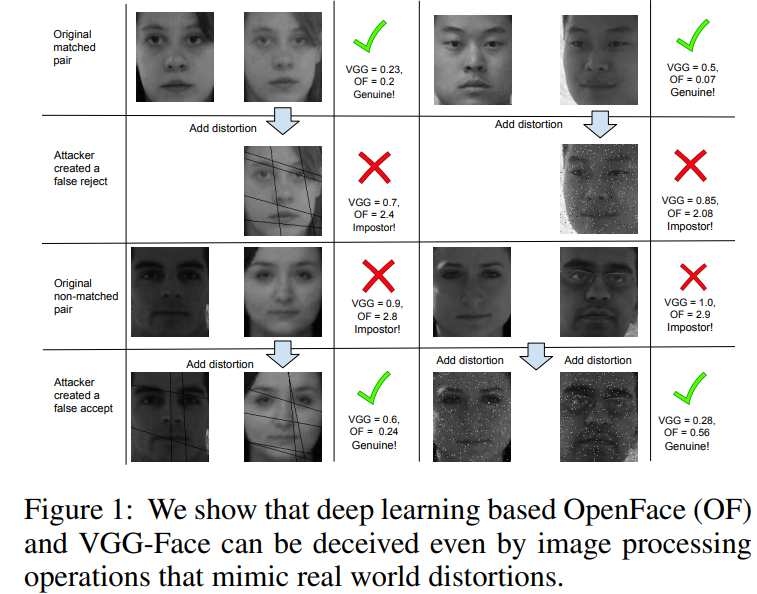
\includegraphics[width=0.90\textwidth]{img/ch4m0.png} 
\caption{ Goswami G 等人 \cite{goswami2018unravelling} }
\label{Test}
\end{figure}

Song Q 等人 \cite{yang2021attacks} 专注于一种对人脸识别网络进行攻击的新颖方法,该方法会误导网络将某人识别为目标人,而不是不明显地错误分类,同时,因为此缘故,研究者引入了一个特定的注意力对抗攻击生成网络来生成假人脸图像。为了捕获目标人的语义信息,这项工作添加了条件变分自动编码器和注意模块来学习人脸之间的实例级对应关系。与传统的双人 GAN 不同,这项工作引入了人脸识别网络作为第三个参与者参与生成器和判别器之间的竞争,这使得攻击者可以更好地模仿目标人。生成的结果难以引起旁观者注意的人脸可以逃避最先进网络的识别,并且大多数人都被识别为目标人。

\begin{figure}[htb]
\centering 
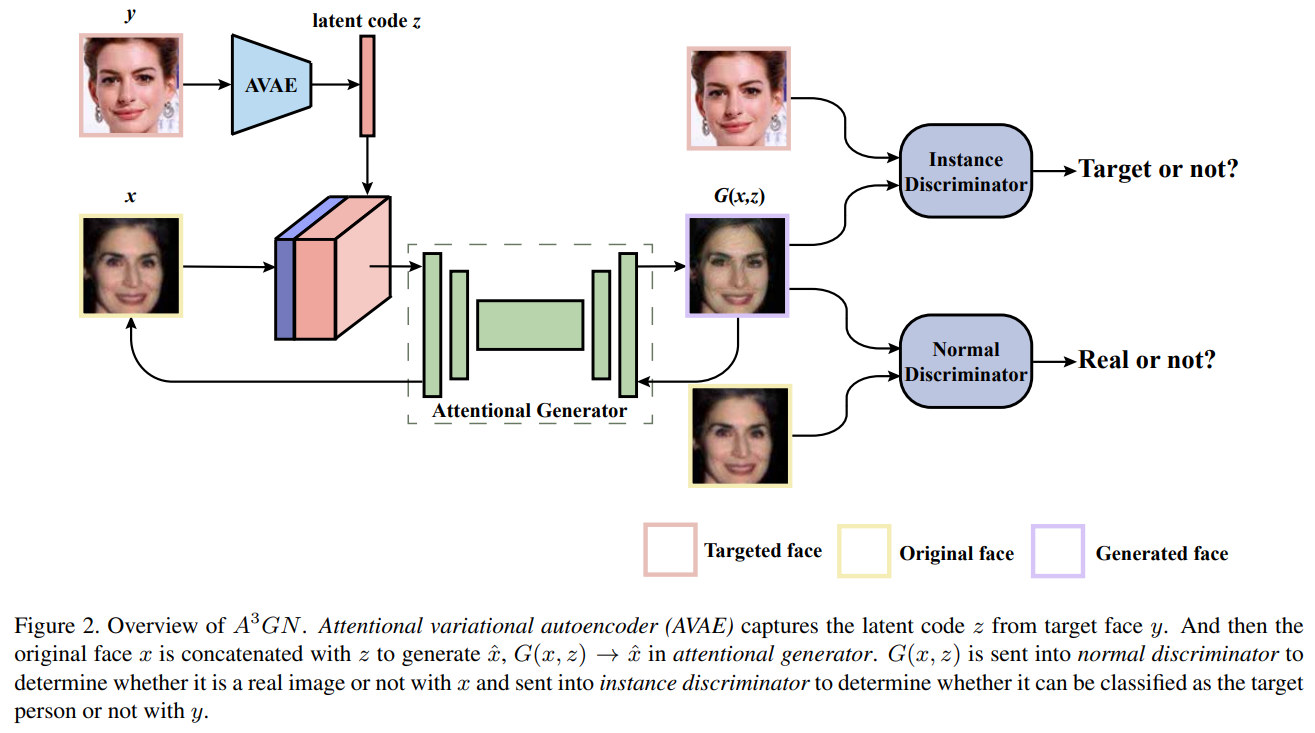
\includegraphics[width=0.90\textwidth]{img/ch4m1.png} 
\caption{ Song Q 等人 \cite{yang2021attacks} }
\label{Test}
\end{figure}

Majumdar P 等人 \cite{majumdar2019evading} 提出了部分面部篡改攻击,其中面部区域被替换或变形以生成篡改样本,而在 CMU-MultiPIE 数据集上使用两个最先进的人脸识别系统 VGG-Face 和 OpenFace 进行的人脸验证实验表明了这些系统对攻击的脆弱性。此外,该研究提出了一种部分人脸篡改检测(PFTD)网络来检测所提出的攻击,该网络通过结合输入图像的原始信息和高频信息来捕获原始图像和篡改图像之间的不一致性,以检测篡改图像。所提出的网络在篡改图像检测方面超越了现有基线深度神经网络的性能。

另外 Korshunov P 等人 \cite{korshunov2018deepfakes},通过使用预先训练的生成对抗网络 (GAN),将视频中的一个人的脸自动替换为另一个人的脸变得越来越容易。最近的公共丑闻,例如,名人的面孔被交换到色情视频上,需要自动检测这些 Deepfake 视频的方法,为了帮助开发此类方法,在本文中,我们展示了第一组从 VidTIMIT 数据库的视频中生成的公开可用的 Deepfake 视频。研究者使用基于 GAN 的开源软件来创建 Deepfakes,该研究强调训练和混合参数可以显著影响结果视频的质量。为了证明这种影响,研究者使用不同调整的参数集生成了具有低和高视觉质量的视频(每个 320 个视频),其研究展示了基于 VGG 和 Facenet 神经网络的最先进的人脸识别系统容易受到 Deepfake 视频的攻击,错误接受率分别为 85.62\% 和 95.00\%,这意味着检测 Deepfake 视频的方法是必要的。通过考虑几种基线方法,我们发现基于口型同步不一致检测的视听方法无法区分 Deepfake 视频。性能最佳的方法,基于视觉质量指标,常用于演示攻击检测领域,在高质量 Deepfakes 上的错误率为 8.97\%,最后的实验表明,GAN 生成的 Deepfake 视频对人脸识别系统和现有检测方法都具有挑战性,而人脸交换技术的进一步发展将使其变得更加困难。同样的也是 Korshunov P 等人 \cite{korshunov2019vulnerability} 展示了 Deepfake 视频的公开数据集,其中的人脸使用基于 GAN 的算法变形,同时为了生成这些影像,研究者使用了基于 GAN 的开源软件,并且我们强调训练和混合参数可以显著影响生成影像的品质,该研究表明,基于 VGG 和 Facenet 神经网络的最先进的人脸识别系统容易受到深度变形视频的影响,错误接受率分别为 85.62 和 95.00,这意味着检测这些视频的方法是必要的。同时研究也考虑了几种检测深度变形的基线方法,并发现基于视觉品质指标的方法(通常用于演示攻击检测领域)导致最佳性能,错误率为 8.97。而最后研究者的实验表明,GAN 生成的深度变形视频对人脸识别系统和现有检测方法都具有挑战性,而深度变形技术的进一步发展将使其更加如此。


\section{深度伪造检测的对抗性}

\section{GAN}

\section{Transformers 與 增量学习}



